%% This is an example first chapter.  You should put chapter/appendix that you
%% write into a separate file, and add a line \include{yourfilename} to
%% main.tex, where `yourfilename.tex' is the name of the chapter/appendix file.
%% You can process specific files by typing their names in at the 
%% \files=
%% prompt when you run the file main.tex through LaTeX.
\chapter{Design}

\begin{figure}[ht!]
	\centering
	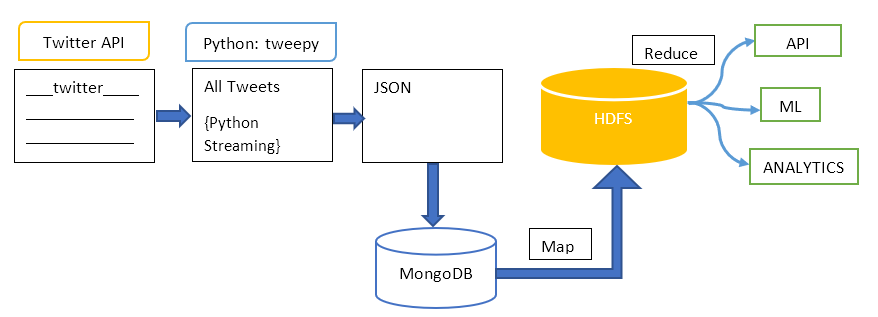
\includegraphics[width=150mm]{DesignDiagram.png}
	\caption{A simple caption \label{overflow}}
\end{figure}

\section{Twitter}

\subsection{Twitter API}\label{ch1:opts}

Twitter as a platform has a lot of users and it generates a lot of data that can be used for analysis. Data can include user tweets, user profiles, user friends and followers, what’s trending, etc. This data can be extracted using twitter Application Programming Interface(API). There are three methods to get this data: the REST API, the search API, and the Streaming API. The Search API is retrospective and allows you search old tweets [with severe limitations], the REST API allows you to collect user profiles, friends, and followers, and the Streaming API collects tweets in real time as they happen. As we are going to do a real time analysis of the data we find the Streaming API most suited to our needs.

The Twitter API requires a few steps:

\begin{enumerate}
  \item Authenticate with OAuth
  \item Make API call
  \item Receive JSON file back
  \item Interpret JSON file
\end{enumerate}

\subsection{Authenticate with OAuth}

OAuth is an open standard for access delegation, commonly used as a way for internet users to grant websites or applications access to their information on other websites or applications access to their information on other websites but without giving them the passwords (Gordon, 2012). Authentication with OAuth on Twitter requires you to get keys from the Twitter developers site using a Twitter developer account. There are four keys (Consumer Key, Consumer Secret Key, Access Token, and Secret Token) that are required to access the API and need to be used during a handshake, once authenticated the program can make API calls.

% This is an example of how you would use tgrind to include an example
% of source code; it is commented out in this template since the code
% example file does not exist.  To use it, you need to remove the '%' on the
% beginning of the line, and insert your own information in the call.
%
%\tagrind[htbp]{code/pmn.s.tex}{Post Multiply Normalization}{opt:pmn}

\subsection{Make API call:}

When making an API call to twitter it has parameters incorporated into the URL, the wrapper looks like this:

\url{https://stream.twitter.com/1.1/statuses/filter.json?track=twitter}

This call is being done through the streaming API, where it is asking to connect to Twitter and once connection is established it will track the keyword ‘twitter’. We can specify our own keywords to track and if we do it carefully we can filter a lot data at an early stage that is irrelevant in our research.

Since, we will be using a python library called tweepy the working of an API call is abstracted from the user, nevertheless understanding the working of the making a Twitter API call is necessary to extract the relevant data.

% This is an example of how you would use tgrind to include an example
% of source code; it is commented out in this template since the code
% example file does not exist.  To use it, you need to remove the '%' on the
% beginning of the line, and insert your own information in the call.
%
%\tgrind[htbp]{code/be.s.tex}{Block Exponent}{opt:be}

\subsection{Receive JSON file back:}

JavaScript Object Notation (JSON) is an open standard file format that has data formatted as attribute-value pairs. The format is language independent and is commonly used for asynchronous browser-server communication for a data request.

JSON files is also the data structure that Twitter returns when an API call is made. The amount of data returned depends how we define our keywords but is usually rather comprehensive and needs to be parsed.

\subsection{Interpret JSON file:}

JSON file can be stored as raw file or can be stored using a SQL/NoSQL database. Since the data received is unstructured the most logical way to store the data would be using a NoSQL database. We will use MongoDB to store the tweets we receive and parse through. We will then run queries based on keywords we need.

\section{Python:}

While there are many different programming languages that can be used to interface with the API, the flexibility and huge community support behind python as well as its relevance in data science makes python the ideal choice for our research. Python has many libraries that has different use cases, we are going to use tweepy to stream our data from twitter.

\section{Tweepy:}

Python is a versatile language with adaptability to various use cases. These are done by extending the language by using libraries which are community created. One of these libraries is tweepy. Tweepy is open-sourced, hosted on GitHub and enables Python to communicate with Twitter platform and use its API (Novalić, 2013). This makes it easier to access the platform to collect and monitor tweets for analysis.

\subsection{Using tweepy:}

Command to install the tweepy library:

\$ pip install tweepy

Tweepy supports OAuth authentication. Authentication is handled by the tweepy.AuthHandler class. (Roesslein, 2011)
A consumer token and a secret key is needed to connect with the twitter stream API, we can use the keys we generated after we created a twitter developer account.

These keys are a pair of private and public (secret and non-secret) keys and used to maintain security. The consumer key pair authorizes your program to use the Twitter API, and the access token essentially signs you in as your specific Twitter user account. This framework makes more sense in the context of third party Twitter developers like TweetDeck where the application is making API calls but it needs access to each user's personal data to write tweets, access their timelines, etc. (Dolinar, 2015)

We can import the tweepy library as below:

\begin{description}
\item[$\bullet$]from tweepy import Stream

\item[$\bullet$]from tweepy import OAuthHandler

\item[$\bullet$]from tweepy.streaming import StreamListener
\end{description}

The above tweepy class imports will be used to construct the stream listener.


\section{Diving into the code:}

\subsection{Importing the modules:}

\begin{figure}[ht!]
	\centering
	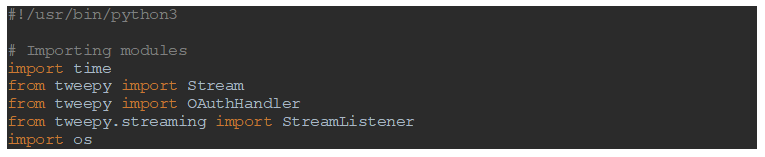
\includegraphics[width=150mm]{code1.png}
	\caption{A simple caption \label{overflow}}
\end{figure}

Apart from the three tweepy class imports that we use to construct the stream listener, the time library will be used to create a time-out feature for the script, and the os library will be used to set your working directory.

\subsection{Setting the Variables:}

\begin{figure}[ht!]
	\centering
	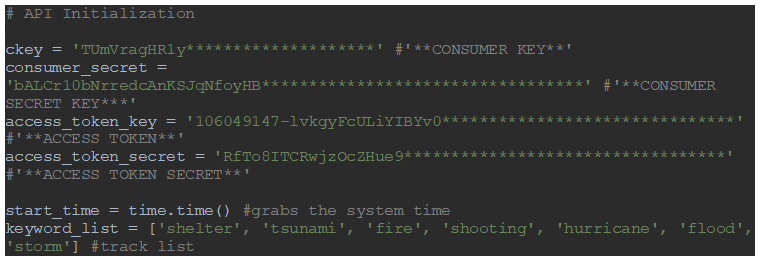
\includegraphics[width=150mm]{code2.png}
	\caption{A simple caption \label{overflow}}
\end{figure}

We have to set the above variables, which will be used in the stream listener by being fed into the tweepy objects.

\subsection{Using and Modifying the Tweepy Classes:}

\begin{figure}[ht!]
	\centering
	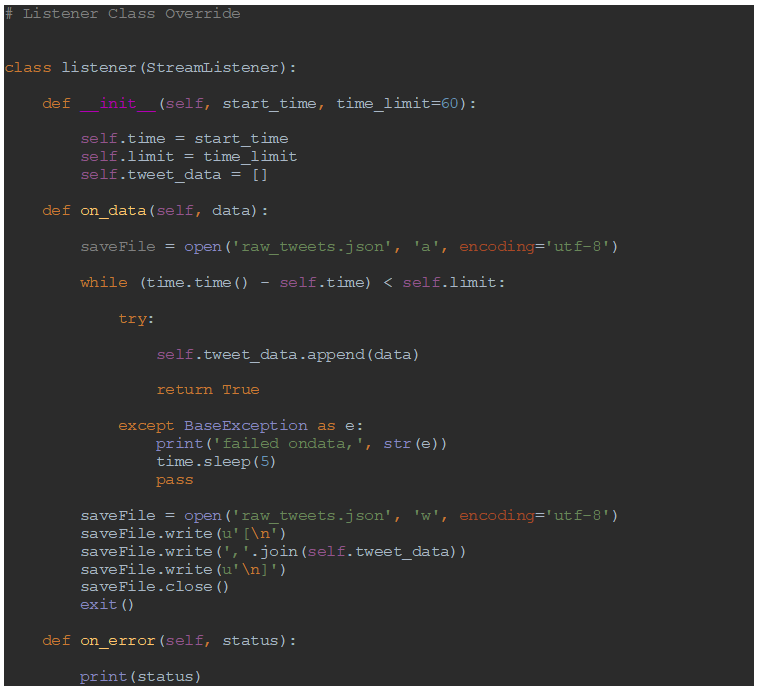
\includegraphics[width=150mm]{code3.png}
	\caption{A simple caption \label{overflow}}
\end{figure}

The code shown below does the following:

\begin{description}
	
\item[$\bullet$]Creates an OAuthHandler instance to handle OAuth credentials

\item[$\bullet$]Creates a listener instance with a start time and time limit parameters passed to it

\item[$\bullet$]Creates an StreamListener instance with the OAuthHandler instance and the listener instance
\end{description}

Before these instances are created, we have to "modify" the StreamListener class by creating a child class to output the data into a .csv file.

We will output the data into MongoDB by reading this csv file.

To elaborate more on the writing of the data to a file after the StreamListener instance receives data:

\begin{figure}[ht!]
	\centering
	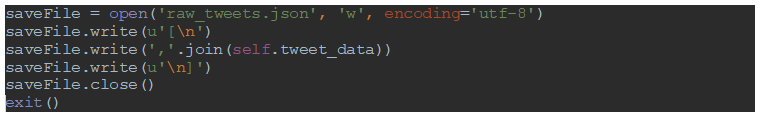
\includegraphics[width=150mm]{code5.png}
	\caption{A simple caption \label{overflow}}
\end{figure}

This block of code opens an output file, writes the opening square bracket, writes the JSON data as text separated by commas, then inserts a closing square bracket, and closes the document. This is the standard JSON format with each Twitter object acting as an element in a JavaScript array. If you bring this into Python built-in parser and the json library can properly handle it.

This section can be modified to or modify the JSON file. For example, we can place other properties/fields like a UNIX time stamp or a random variable into the JSON. We can also modify the output file or eliminate the need for a .csv file and insert the tweet directly into a MongoDB database. As it is written, this will produce a file that can be parsed by Python's json class.

After the child class is created we can create the instances and start the stream listener.

\subsection{Calling the Stream Listener:}

\begin{figure}[ht!]
	\centering
	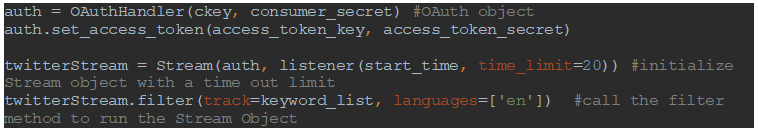
\includegraphics[width=150mm]{code6.png}
	\caption{A simple caption \label{overflow}}
\end{figure}

Here the OAuthHandler uses your API keys [consumer key and consumer secret key] to create the auth object. The access token, which is unique to an individual user [not an application], is set in the following line. This will take all four of your credentials from the Twitter Dev site. The modified StreamListener class simply called listener is used to create a listener instance. This contains the information about what to do with the data once it comes back from the Twitter API call. Both the listener and auth instances are used to create the Stream instance which combines the authentication credentials with the instructions on what to do with the retrieved data. The Stream class also contains a method for filtering the Twitter Stream. The parameters are passed to the Stream API call.

\section{MongoDB}

Storing JSON tweets as a .csv file works well, but they don’t always make good flat .csv files as not every tweet has the same structure nor do every tweet contain the same fields. Some data is well nested into the JSON objects. It is possible to write a parser that has a field for each possible subfield, but this can take a lot of time as involves a lot of considerations and will also create a large .csv file or SQL database.

NoSQL databases like MongoDB greatly simply tweet storage, search and recall which eliminates the need to use an extensive tweet parser.

\subsection{What is MongoDB?}

It is a document-based database that stores data using documents rather than using tuples in tables like traditional relational databases. These documents are similar in structure to JSON objects using key-value pairs and are called BSON (Binary JSON). JSON and BSON have similar properties as JS objects and Python dictionaries.

\subsection{Why store in MongoDB?}

Storing tweets in MongoDB makes sense as BSON and JSON are so similar and that makes putting the entire content of a tweet’s JSON string into an insert statement and executing that statement to store the data. This also makes recalling and searching for tweets simple although it does require a change in thought process of rather executing traditional SQL commands to treating data as OOP structures.

\section{Storing Tweets in MongoDB:}

\begin{figure}[ht!]
	\centering
	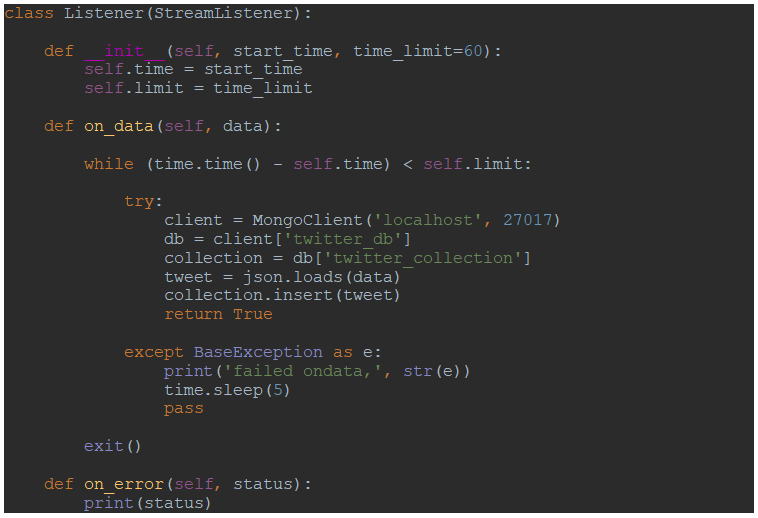
\includegraphics[width=150mm]{code7.png}
	\caption{A simple caption \label{overflow}}
\end{figure}

Once MongoDB is installed and configured storing tweets is simple using the Python stream listener. Modifying the code shown above we have to import pymongo and json libraries. The json library is the default python library and will be available to import, pymongo needs to be set up using the following command:

\$ pip install pymongo

The main changes in the code that I had to do was in the listener child class as shown below.

$MongoClient creates the MongoClient instance which interfaces with the database. The client[‘twitter_db’] call designates the database that is going to be used, and the db[‘twitter_collection’] call selects the collection where the documents will be stored. The json.loads() call converts the string returned from the Twitter API into a json object in Python. Finally, the collection.insert() call inserts the json object into the MongoDB database. From this rather simple change to the Python stream listener all the tweets can be saved into a MongoDB database.
$
\section{Recalling Tweets from MongoDB:}

The function to retrieve any document from a MongoDB database is collection.find(). Here, I can specify what I want or leave it black to get all the documents returned, in my case it will be all the tweets.

Calling using the .find() method, Python returns a MongoDB cursor, which can be iterated through by putting it in a for loop. The for loop will run the loop for each object in the iterator. 

\section{Hadoop:}